\documentclass[11pt,letterpaper]{article}
\usepackage[margin=1in]{geometry}
\usepackage[T1]{fontenc}
\usepackage{lmodern,microtype,amsmath,amssymb,amsthm,booktabs,array,longtable,graphicx,enumitem,xurl}
\usepackage[hidelinks]{hyperref}
\setlist{nosep,leftmargin=*}
\newtheorem{proposition}{Proposition}
\newtheorem{remark}{Remark}
\newcommand{\D}{D^\star}
\title{From deformation costs to conditional expression intervals}
\author{GeoCert-ST research extension and executable handoff}
\date{28 October 2026}
\begin{document}\maketitle
\begin{abstract}
We implement hard-budget expression-count intervals on the existing ordered-corridor uncertainty model. Exact targeted enumeration uses source-admissible pinned reconstruction; a second method computes sound Lagrangian bounds with integer rounding, witnesses and explicit gaps. The native census contains 6,326 local cell--gene interval functions across 84 corridor/setting models. Five illustrative budgets produce 31,630 intervals. All tested dual endpoints match exact enumeration, although a two-transcript example proves that duality can fail in general. Standard residual-cut theory also supplies a compact representation of all penalized optima. These are conditional geometric certificates on the existing single-donor development data. They do not establish realistic error budgets, anatomical accuracy, statistical coverage, or a whole-slide method.
\end{abstract}

\section{The quantity now computed}
Fix one corridor $\mathcal C$, its geometric settings $\theta$, and its finite feasible ownership vectors $\mathcal F$. The previous representation theorem gives the exact minimum continuous deformation $\D(c)$ for each $c\in\mathcal F$, together with a realizing boundary. For a gene $g$ and cell $k$, let
\[
 Q(c)=q_{\rm outside}+\sum_{i\in I_g} w_i\mathbf1[c_i=k],\qquad w_i\in\mathbb Z_{>0}.
\]
The offset counts retained transcripts in the cell outside the modeled sites; those assignments are fixed. In the native analysis each site has weight one. For a declared area budget $\delta\ge0$, define
\[
 \mathcal F_\delta=\{c\in\mathcal F:\D(c)\le\delta\},\qquad
 L(\delta)=\min_{\mathcal F_\delta} Q(c),\quad U(\delta)=\max_{\mathcal F_\delta} Q(c).
\]
An empty $\mathcal F_\delta$ is reported as empty, not as an expression interval. Every count realized by a feasible continuous boundary in the budget lies in $[L,U]$: its assignment has minimum deformation no larger than the boundary's actual deformation. Conversely, an attaining canonical boundary realizes each computed endpoint. The guarantee is deterministic, conditional on the family. It is neither a confidence interval nor a posterior credible interval.

\begin{figure}[!htbp]\centering
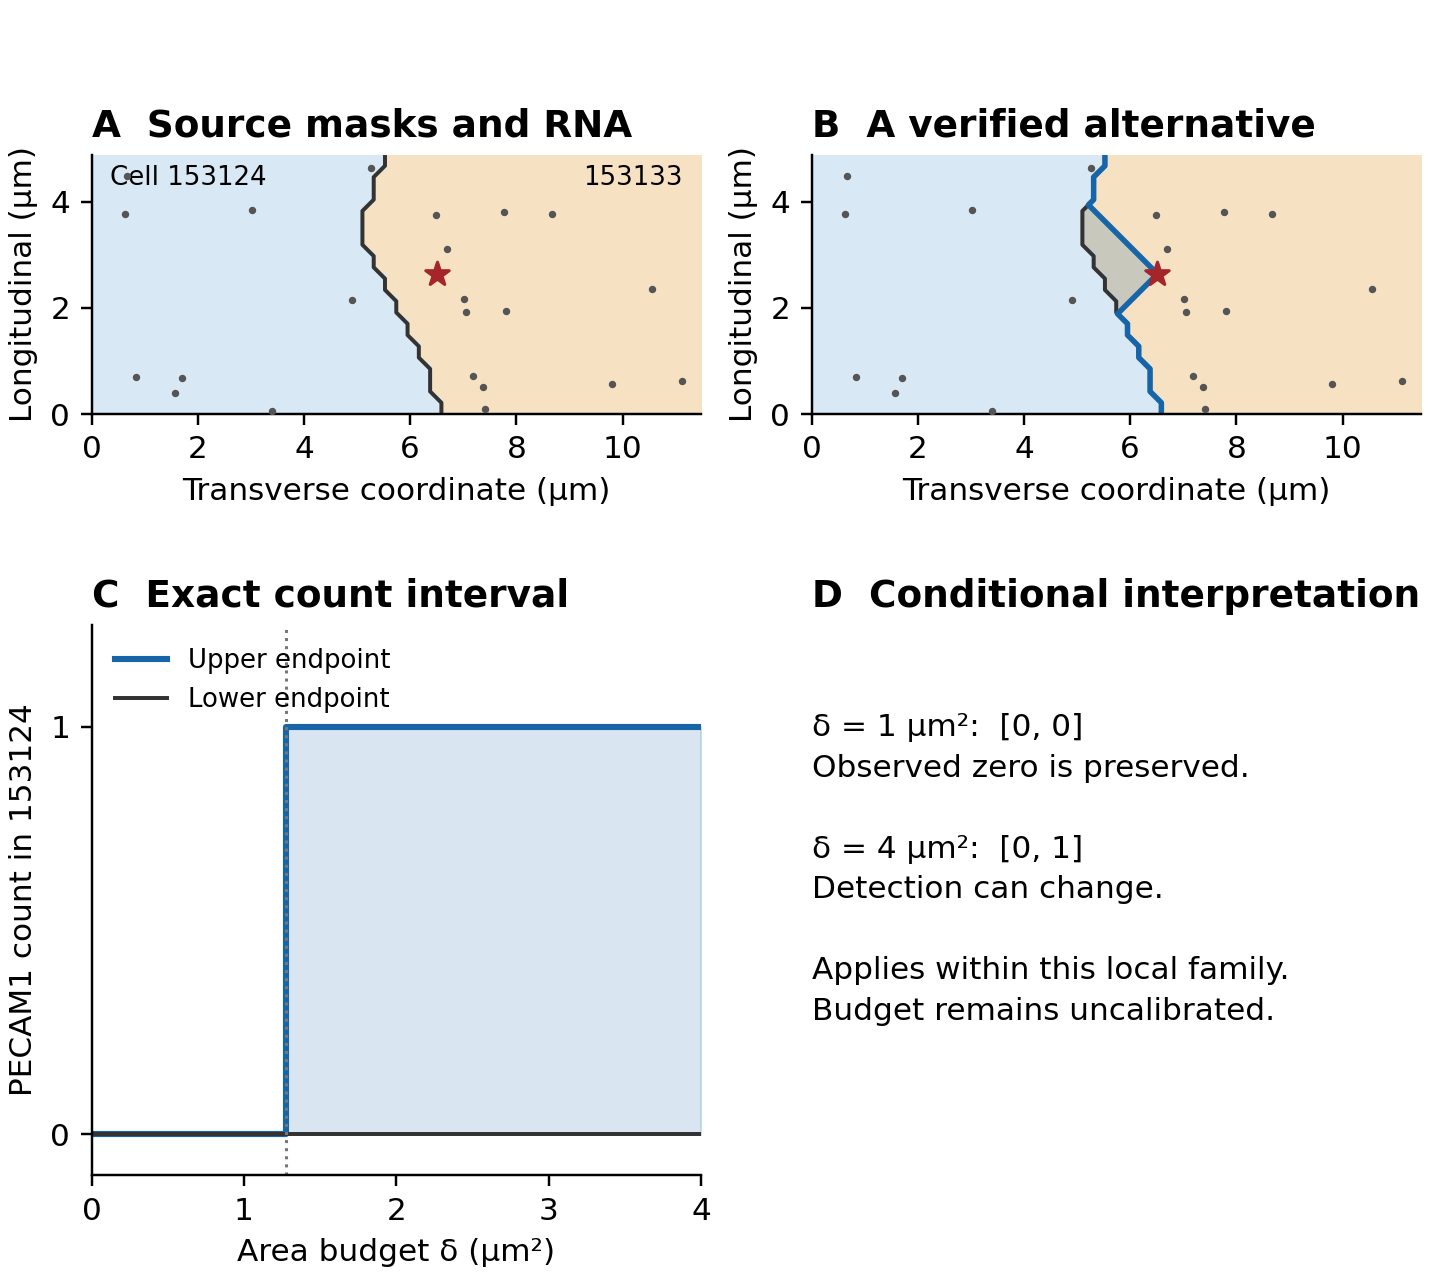
\includegraphics[width=\linewidth]{budget_story.png}
\caption{An existing baseline corridor connects supplied source masks, a verified boundary alternative, and an observed-count interval. The star is PECAM1. The alternative has minimum deformation approximately $1.277468\,\mu\mathrm m^2$. At budget one, the target cell's observed zero is invariant within this family; at budget four, it can become one. The displayed crop is a local mask patch, not new microscopy or new tissue. Other crop assignments stay fixed.}
\end{figure}

\section{Sound cut bounds, with the rounding direction stated}
For $\mu\ge0$, compute with the ownerwise cut representation
\[
 A_-(\mu)=\min_{c\in\mathcal F}\{\mu\D(c)-Q(c)\},\qquad
 A_+(\mu)=\min_{c\in\mathcal F}\{\mu\D(c)+Q(c)\}.
\]
The fixed offset may be carried outside the graph. The implementation does so explicitly.
\begin{proposition}[Integer outer bounds]
For every nonempty budget family and any finite nonempty multiplier set $M\subseteq[0,\infty)$,
\[
 \max_{\mu\in M}\left\lceil A_+(\mu)-\mu\delta\right\rceil
 \ \le L(\delta)\le U(\delta)\le
 \min_{\mu\in M}\left\lfloor\mu\delta-A_-(\mu)\right\rfloor.
\]
\end{proposition}
\begin{proof}
For any budget-feasible $c$, $A_-(\mu)\le\mu\D(c)-Q(c)\le\mu\delta-Q(c)$, giving the upper inequality. Also $A_+(\mu)\le\mu\D(c)+Q(c)$ implies $Q(c)\ge A_+(\mu)-\mu\D(c)\ge A_+(\mu)-\mu\delta$. Counts are integers, so floor the upper bound and ceil the lower bound. Intersecting bounds preserves validity.
\end{proof}
Every cut result includes an integer flow/cut certificate and a checked rational boundary. A cut optimizer need not satisfy the budget. The software retains only budget-feasible outputs as witnesses. It reports
\[
 \underline L\le L\le L_{\rm witness},\qquad
 U_{\rm witness}\le U\le\overline U,
\]
with two endpoint gaps. Equality with the corresponding witness proves exactness. Arbitrary feasible optimization outputs alone do not prove an outer bound: the dual objective needs a certified optimum, or a certified lower bound on its minimization problem.

\section{Exact endpoints by targeted enumeration}
The previous pinned-query theorem applies when the source satisfies every source-owner obligation and structural pin at zero deformation. Its implementation checks that premise. Let $G$ contain exactly the RNA groups contributing to $Q$. For each $i\in G$, compute the individually feasible owner set $A_i$ using implication closure. Enumerate $\prod_{i\in G}A_i$. For each feasible choice $a$, pin these owners and use the source-clipping algorithm to obtain the minimum deformation over every completion of the other owners. Store the smallest cost for each resulting integer count.
\begin{proposition}[Complete count frontier]
Under the source-admissibility premise, the procedure returns
\[
 d_q=\min\{\D(c):c\in\mathcal F,\ Q(c)=q\}
\]
for every attainable count $q$. Consequently $L(\delta)=\min\{q:d_q\le\delta\}$ and $U(\delta)=\max\{q:d_q\le\delta\}$ for every nonnegative budget.
\end{proposition}
\begin{proof}
Every full feasible vector restricts to one enumerated target-owner choice. Conversely, every retained choice has a feasible completion, whose count is determined by the pinned target groups. The pinned-query theorem minimizes deformation over all those completions. Taking the minimum over choices with the same count therefore equals the minimum over the full set of feasible vectors with that count. Canonical reconstruction provides an attaining boundary.
\end{proof}
The enumeration factor is $\prod_i|A_i|$, exponential in the number of relevant transcript groups in the worst case. The code enforces a cap and refuses to label truncated enumeration complete. This is a useful algorithm for sparse local gene queries, not a general polynomial hard-budget solver. In this native census the largest target enumeration has only eight combinations. It would be misleading to argue that these count queries inherently need the full integrated-cost graph.

\section{Penalty paths, all optima, and the tractability boundary}
\paragraph{Implemented supported paths.}
For a signed integer reward $R(c)$, the oracle minimizes $\mu\D(c)-R(c)$. The implementation supports counts and integer linear count contrasts. Let $W$ bound the reward range, let $B$ bound the deformation range, and let $H$ be a common denominator of all integrated area coefficients. A query at $\mu=1/(B+1)$ obtains maximum reward with least deformation. A query at $\mu=(W+1)H$ obtains minimum deformation with maximum reward. The score gap is at least one and the positive area gap at least $1/H$, proving these lexicographic choices.

Between frontier points $(d_a,r_a)$ and $(d_b,r_b)$, query $\mu=(r_b-r_a)/(d_b-d_a)$. If the oracle lies strictly below their common supporting line, recurse on the two subintervals; otherwise the chord is supported. This finite dichotomic construction supplies all supporting breakpoints needed for the optimal Lagrangian bound. A call cap retains sound partial bounds and sets \texttt{complete=false}. It does not recover unsupported budget optima.

\paragraph{When nesting is available.}
The classical monotone parametric-flow conditions require source capacities moving in one direction, sink capacities in the opposite direction, and fixed internal capacities~\cite{ggt}. They cannot be assumed merely because a problem is graph-representable. For $\mu>0$, divide by $\mu$ and write $D-\tau Q$, $\tau=1/\mu$. Counting an exterior cell produces threshold-bit coefficients of one polarity, supplying a standard sufficient condition for nested extremal cuts (with hard implications treated as infinite). Counting an interior ordered cell involves a difference of adjacent threshold bits, with mixed signs; the same condition need not hold. The current code uses repeated verified cuts, not a Gallo--Grigoriadis--Tarjan implementation or a claimed one-flow runtime.

\paragraph{Every penalized optimal assignment.}
Given a verified maximum flow, retain forward residual arcs with unused capacity and reverse arcs carrying positive flow. Contract their strongly connected components. Successor-closed component sets containing the source component and excluding the sink component represent all minimum cuts~\cite{pq}. Projection through the contraction map onto the original owner bits represents all optimal owner vectors; different auxiliary cuts may project to the same vector. The implementation supplies this DAG, forced components, possible owners, and bounded enumeration for testing. Possible owners at different groups are dependent. This representation describes penalized optima, not all budget-feasible assignments or all continuous realizing boundaries.

\paragraph{A proved obstruction to the proposed shortcut.}
In the existing two-site tent model, the minimum deformation at count $0,1,2$ is $0,1/16,7/64$. At budget $\delta=3/50$, the exact maximum is zero. The best continuous dual value is
\[
 \inf_{\mu\ge0}\left\{\mu\delta+\max(0,1-\mu/16,2-7\mu/64)\right\}
 =\frac{192}{175}.
\]
It is attained at $\mu=128/7$ and rounds down to one, leaving a strict integer gap. At $\delta=1/16$, count one is an exact budget optimum but is never a penalized optimum: at the only possible transition, counts zero and two tie and count one is worse. The residual DAG recovers precisely both tied vectors.

\paragraph{What has not been proved.}
Graph representability alone does not make the general hard-budget problem polynomial: independent unary costs $D(x)=\sum_i a_ix_i$ and rewards $R(x)=\sum_i v_ix_i$ give the $0/1$ knapsack problem under $D(x)\le\delta$. This observation is not a hardness reduction for the specific continuous GeoCert family. Nor does the usual three-terminal hardness statement immediately establish hardness of planar tessellations: planar multiway cut is polynomial for fixed terminal count and NP-hard when the count is part of the input~\cite{multiway}. A geometric reduction must preserve its topology, admissibility and cost. Star-shaped cells, tree adjacency and layered 3D domains remain research candidates, not implemented tractable classes. The nearest-clamp argument is dimension-independent when feasible envelopes and min/max closure hold, but exact integration and a polynomial representation require separate analysis in a new domain.

\section{Executed results and their limits}
All original 42 corridors and both settings are retained. We include every gene observed in a relevant source cell or retained corridor site. Sparse zero defaults apply only within the released observed-gene vocabulary; the CLI rejects unknown genes rather than interpreting unmeasured genes as absent. The 2,832 model--gene enumerations check 3,077 owner combinations and yield 6,326 cell--gene interval functions. Only 401 functions can vary under the full geometric family. They are overlapping local calculations, not independent biological replicates or a stitched segmentation.

\begin{center}\begin{tabular}{lrr}\toprule
Five-budget census & Baseline & Relaxed family\\\midrule
Cell--gene--budget rows &15,815&15,815\\
Nondegenerate exact intervals &322&1,009\\
Joint interval tighter than singleton enclosure &0&5\\\bottomrule
\end{tabular}\end{center}
The illustrative budgets are $0,1/4,1,4,16\,\mu\mathrm m^2$. They were not estimated from segmentation errors. Across this grid, all 31,630 Lagrangian endpoint bounds equal the exact endpoints; additional frontier and midpoint checks give 32,506 soundness comparisons. Some are fixed by feasibility and need no cut. The 401 variable functions require 2,857 penalized cut calls in this implementation.

\paragraph{The singleton comparator is sound.}
For each RNA, retain every owner whose exact pinned minimum cost is at most $\delta$. Optimize that RNA's count contribution independently and sum the extrema. Every jointly budget-feasible assignment passes these individual tests, so the resulting interval is an outer enclosure, although its endpoints need not be jointly attainable. The joint intervals improve it in five relaxed-family rows, spanning three corridors (CAVIN1, TNFRSF17 and CPA3). No baseline-grid improvement is observed. This null result remains important: the new question is useful, but the existing native genes are sparse and the stronger joint machinery has limited observed advantage here.

\paragraph{Validation scope.}
Twenty generated small models check count and signed-contrast frontiers against complete full-owner enumeration, with 162 budget comparisons and 81 feasible full-owner states. Residual-DAG projection agrees on 33 optimal vectors. The native showcase contributes 38 gene--cell frontiers checked against the archived independent scalar calculation of all 26 feasible owner costs. Tests also cover a positive mandatory deformation, rejection of an invalid source-clipping premise, enumeration limits, and incomplete-path status. These are computational checks, not human proof review or new biological ground truth.

\section{Downstream conclusions and probability}
For one common uncertainty family, $L_g>0$ certifies retained-gene detection throughout that family, while $U_g=0$ certifies an observed zero. Two positive lower bounds certify simultaneous detection; positive upper bounds alone do not prove that both can be attained together. Signed integer linear contrasts are supported by the same cut-bound and targeted-enumeration logic. An interval excluding zero certifies the sign of that descriptive contrast. Differential-expression $p$-values, FDR control, ratios with changing denominators, cell-type labels, and ligand--receptor activity require additional statistical or biological models.

\paragraph{Calibration is a separate task.}
The utility \texttt{core/calibration.py} implements the split-conformal order statistic $\lceil(n+1)(1-\alpha)\rceil$, checks unit identifiers for overlap, and abstains when a finite threshold is unavailable~\cite{conformal}. No tissue data have been fitted with it. A valid deployment needs geometry fixed on training donors, scores on exchangeable independent calibration units, and a declared simultaneous-versus-marginal coverage target. Scores must account for violations of the geometric family, not merely area differences among accepted cases. Serial sections are not automatically paired ground truth for the same cells. A marginal donor-level guarantee is not conditional coverage for every cell and gene.

\paragraph{MAP does not imply a marginal posterior.}
A specified finite-dimensional model may use a density proportional to $\exp[-\lambda D(f)-C(c)]$. Minimizing over $f$ gives a profile/MAP energy; marginalizing requires an integral over all compatible boundaries and includes volume factors. On an infinite-dimensional boundary space, even the reference measure must be specified. One can separately define a finite owner Gibbs law using $\D(c)$, but this is a modeling choice. Unary perturb-and-MAP generally approximates rather than exactly samples a discrete Gibbs law~\cite{pm}.

The executable diagnostic uses two coincident sites, so only two joint owners are feasible, with energies zero and one. Their exact non-source Gibbs probability is approximately $0.26894$. In 2,000 seeded unary-Gumbel perturbations, the non-source frequency is $0.3415$, with Wilson 95\% Monte Carlo interval $[0.3210,0.3626]$. Every sampled boundary is feasible and optimal for its quantized perturbed energy. The discrepancy concerns the sampling law: exact MAP optimization does not make the samples exact Gibbs draws. This is a synthetic diagnostic, not a biological posterior experiment.

\section{Corrections to the proposed research agenda}
Uncertainty-aware spatial expression and downstream inference already have substantial prior work; TISSUE treats imputation uncertainty rather than this segmentation-family question~\cite{tissue}. Historical priority for geometric count certificates has not been established. XIST in a male cell is not a misassignment by definition: male-cancer expression has been documented~\cite{xist}. Species and reporter probes can provide strong orthogonal evidence, but require validated specificity, independent cell labels, and controls for ambient RNA, transfer and mixed material. Marker exclusivity is a proxy, not universally valid ground truth.

The next study should freeze extraction, uncertainty families, budget calibration and endpoints before opening held-out outcomes. Compare interval width and coverage, plus error ranking where transcript ownership labels are credible. Report all exclusions and out-of-family samples. Compare methods only on compatible tasks: a deterministic interval, a segmentation, a posterior estimate and an overlap diagnostic are different outputs. Use donors as biological replication units; repeated corridors and penalties do not supply independent samples. This release makes no new AUROC, calibration, DE-FDR or whole-slide timing claim.

\paragraph{Engineering boundary.}
The current code uses Python's standard library for exact computation. There is no Rust/C++ backend, general SpatialData importer, napari plugin or million-cell benchmark. Global relaxation requires a model whose projections provably contain the full-tissue possibilities and whose cost accounting treats shared boundaries consistently. Independently fixing the exterior of overlapping corridors does not meet that requirement. A faster max-flow backend alone would not resolve this geometry problem.

\section{Files and continuation}
The full source archive includes the earlier manuscript and supplement, source crops, exact inputs, previous artifacts, new code/tests, interval records and this note. Start with \texttt{START\_HERE.txt} and \texttt{NEXT\_CHAT\_PROMPT.txt}. The previous ten-page submission manuscript has not been silently rewritten around uncalibrated new claims. The new experiment is an executed research extension for review and integration.
\begin{verbatim}
python tests/test_budget_counts.py
python geocert_counts.py interval --corridor 4037abe9fea38e \
  --cell 153124 --gene PECAM1 --budget 1 --output run/count.json
python geocert_counts.py verify run/count.json
python experiments/budget_census.py --output-dir run/budgets
python experiments/perturb_map_diagnostic.py --samples 2000
\end{verbatim}
The same query with \texttt{--method dual} emits all cut proofs, paths, witnesses and remaining gaps. \texttt{results/budgets/native\_frontiers.json.gz} contains complete count frontiers and exact boundary witnesses; \texttt{native\_intervals.csv} is the illustrative grid. The census stores compact dual path values; individual commands regenerate their complete flow certificates. AI assisted implementation, analysis and writing. Human authors remain responsible for checking the arguments, interpreting the data and accurately describing the assistance.

\clearpage
\begin{thebibliography}{9}
\bibitem{pq} J.-C. Picard and M. Queyranne. On the structure of all minimum cuts in a network and applications. \emph{Mathematical Programming Studies} 13:8--16, 1980. \url{https://doi.org/10.1007/BFb0120902}.
\bibitem{ggt} G. Gallo, M. D. Grigoriadis and R. E. Tarjan. A fast parametric maximum flow algorithm and applications. \emph{SIAM J. Comput.} 18(1):30--55, 1989. \url{https://doi.org/10.1137/0218003}.
\bibitem{multiway} E. Dahlhaus et al. The complexity of multiterminal cuts. \emph{SIAM J. Comput.} 23(4):864--894, 1994. \url{https://doi.org/10.1137/S0097539792225297}.
\bibitem{pm} G. Papandreou and A. L. Yuille. Perturb-and-MAP random fields: using discrete optimization to learn and sample from energy models. \emph{ICCV}, 2011. \url{https://doi.org/10.1109/ICCV.2011.6126242}.
\bibitem{conformal} A. N. Angelopoulos and S. Bates. A gentle introduction to conformal prediction and distribution-free uncertainty quantification. arXiv:2107.07511, 2021. \url{https://arxiv.org/abs/2107.07511}.
\bibitem{tissue} E. D. Sun et al. TISSUE: uncertainty-calibrated prediction of single-cell spatial transcriptomics improves downstream analyses. \emph{Nature Methods} 21:444--454, 2024. \url{https://doi.org/10.1038/s41592-024-02184-y}.
\bibitem{xist} A. Sadagopan et al. Somatic XIST activation and features of X chromosome inactivation in male human cancers. \emph{Cell Systems} 13(11):932--944.e5, 2022. \url{https://doi.org/10.1016/j.cels.2022.10.002}.
\end{thebibliography}
\end{document}
